\subsubsection{UC1 - Autenticazione}\label{UC1}

\begin{figure}[H]
  \centering
  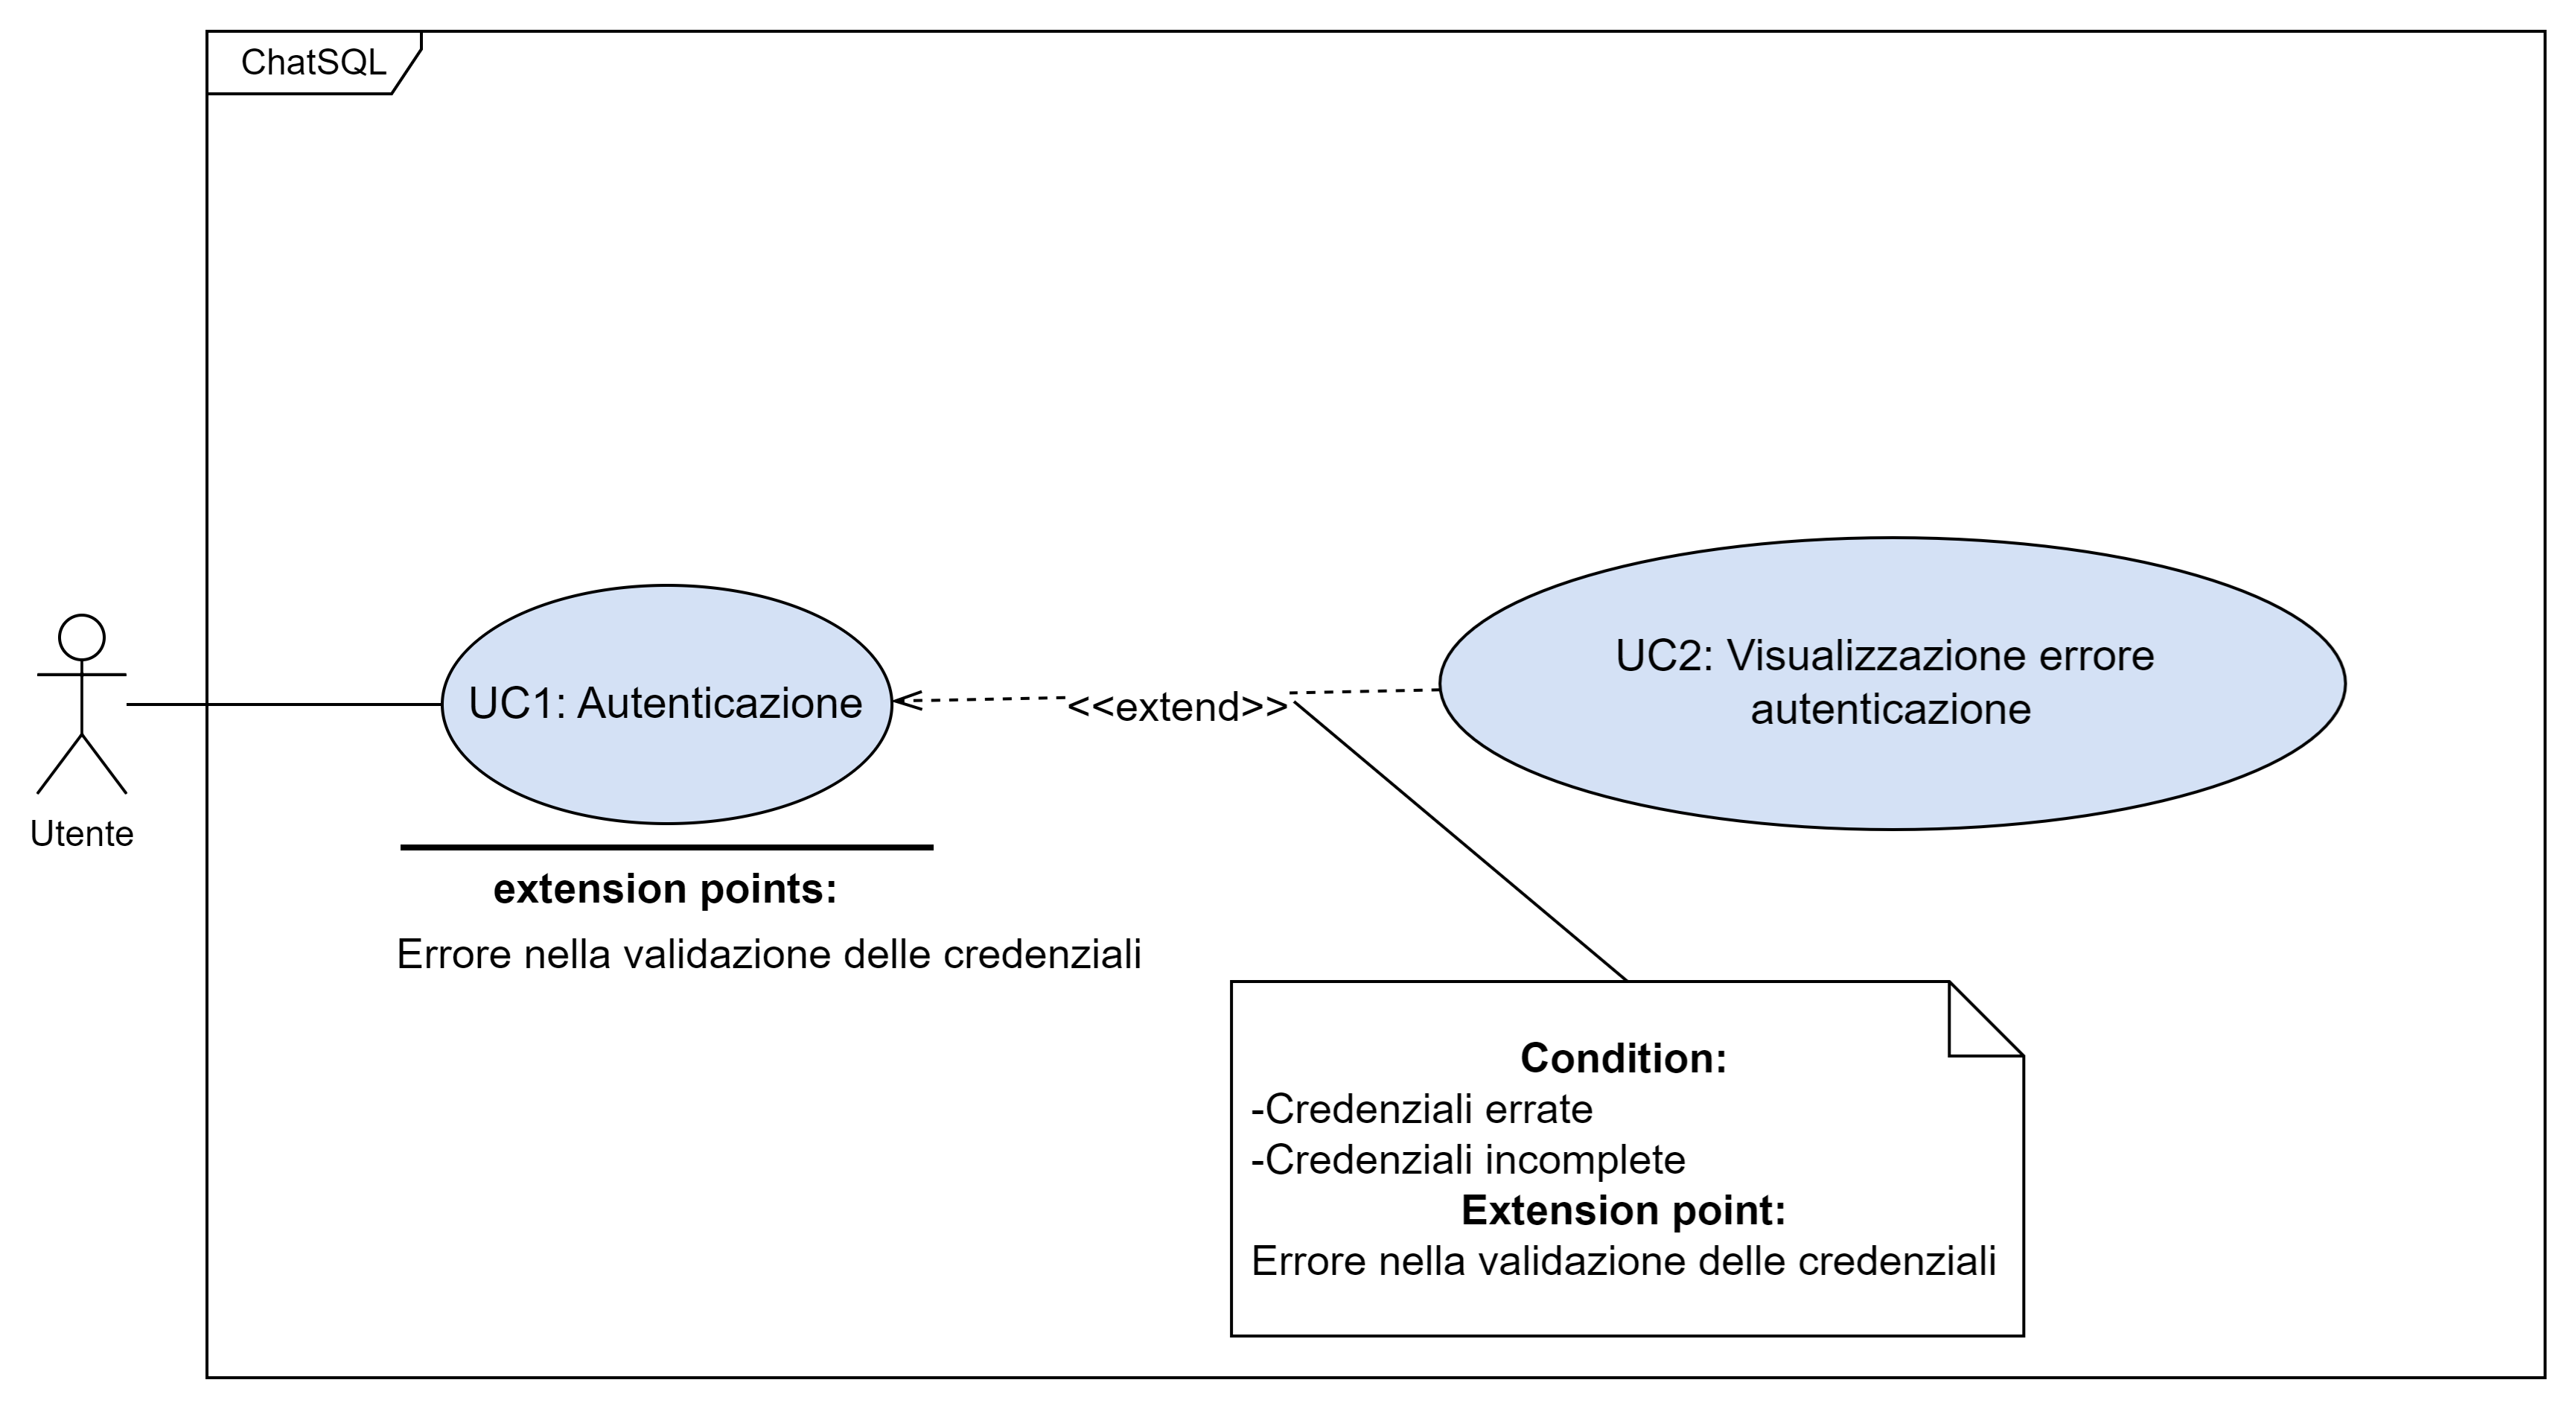
\includegraphics[width=0.90\textwidth]{assets/uc1.png}
  \caption{UC1}
\end{figure}

\paragraph*{Descrizione}
L’Autenticazione corrisponde al processo di login, tramite il quale l'Utente può passare alle funzionalità del Tecnico.

\paragraph*{Attori principali}
Utente

\paragraph*{Precondizioni}
\begin{itemize}
  \item L’Utente si collega all’applicativo;
  \item L'Utente non è già autenticato nella sessione corrente;
  \item L’Utente ha avviato la procedura di login all’applicativo.
\end{itemize}

\paragraph*{Postcondizioni}
\begin{itemize}
  \item La procedura di autenticazione si è conclusa con successo;
  \item L’Utente diventa Tecnico;
  \item Il Tecnico visualizza le funzionalità aggiuntive specifiche del ruolo.  
\end{itemize}

\paragraph*{Scenario principale}
\begin{itemize}
  \item L’Utente accede all’applicativo;
  \item L’Utente seleziona la funzione di login;
  \item L’Utente inserisce le proprie credenziali di accesso;
  \item In caso di corretto inserimento e verifica delle credenziali, l’Utente accede all’applicativo come Tecnico.
\end{itemize}

\paragraph*{Scenario alternativo}
\begin{enumerate}
  \item Il sistema riconosce un errore durante il tentativo di autenticazione da parte dell'Utente (\hyperref[UC2]{UC2});
  \item Viene visualizzato un messaggio con i dettagli dell'errore.
\end{enumerate}

\paragraph*{Estensioni}
\begin{itemize}
  \item Errore per fallita autenticazione (\hyperref[UC2]{UC2}).
\end{itemize}

\paragraph*{Inclusioni}
\begin{itemize}
  \item Inserimento e-mail (\hyperref[UC1point1]{UC1.1});
  \item Inserimento password (\hyperref[UC1point2]{UC1.2}).
\end{itemize}

%%%%%%%%%%%%%%%%%%%%%%%%%%%%%%%%%%%%%%%%%%%%%%%%%%%%%%%%%%%%%%%%%%%%%%%%%%%%%%

\subsubsection{UC1.1 - Inserimento e-mail}\label{UC1point1}

\paragraph*{Descrizione}
La procedura di inserimento e-mail corrisponde all’inserimento della propria e-mail nella sezione apposita di login.

\paragraph*{Attori principali}
Utente

\paragraph*{Precondizioni}
\begin{itemize}
  \item L’Utente non ha eseguito il login;
  \item L’Utente ha avviato la procedura di autenticazione.  
\end{itemize}

\paragraph*{Postcondizioni}
\begin{itemize}
  \item L’Utente ha correttamente inserito la propria e-mail nel campo apposito.
\end{itemize}

\paragraph*{Scenario principale}
\begin{enumerate}
  \item L’Utente avvia la procedura di autenticazione;
  \item L’Utente inserisce la propria e-mail nel campo apposito.  
\end{enumerate}

%%%%%%%%%%%%%%%%%%%%%%%%%%%%%%%%%%%%%%%%%%%%%%%%%%%%%%%%%%%%%%%%%%%%%%%%%%%%%%

\subsubsection{UC1.2 - Inserimento password}\label{UC1point2}
\paragraph*{Descrizione}
La procedura di inserimento password corrisponde all’inserimento della password dell'Utente nella sezione apposita di login.

\paragraph*{Attori principali}
Utente

\paragraph*{Precondizioni}
\begin{itemize}
  \item L’Utente non ha eseguito il login;
  \item L’Utente ha avviato la procedura di autenticazione (\hyperref[UC1]{UC1});
  \item L’Utente ha inserito la propria e-mail nel campo apposito (\hyperref[UC1point1]{UC1.1}).
\end{itemize}

\paragraph*{Postcondizioni}
\begin{itemize}
  \item L’Utente ha correttamente inserito la propria password nel campo apposito.
\end{itemize}

\paragraph*{Scenario principale}
\begin{enumerate}
  \item L’Utente avvia la procedura di autenticazione;
  \item L’Utente inserisce la propria e-mail nel campo apposito; 
  \item L’Utente inserisce la propria password nel campo apposito.  
\end{enumerate}
